\begin{figure}[h]
  \centering
  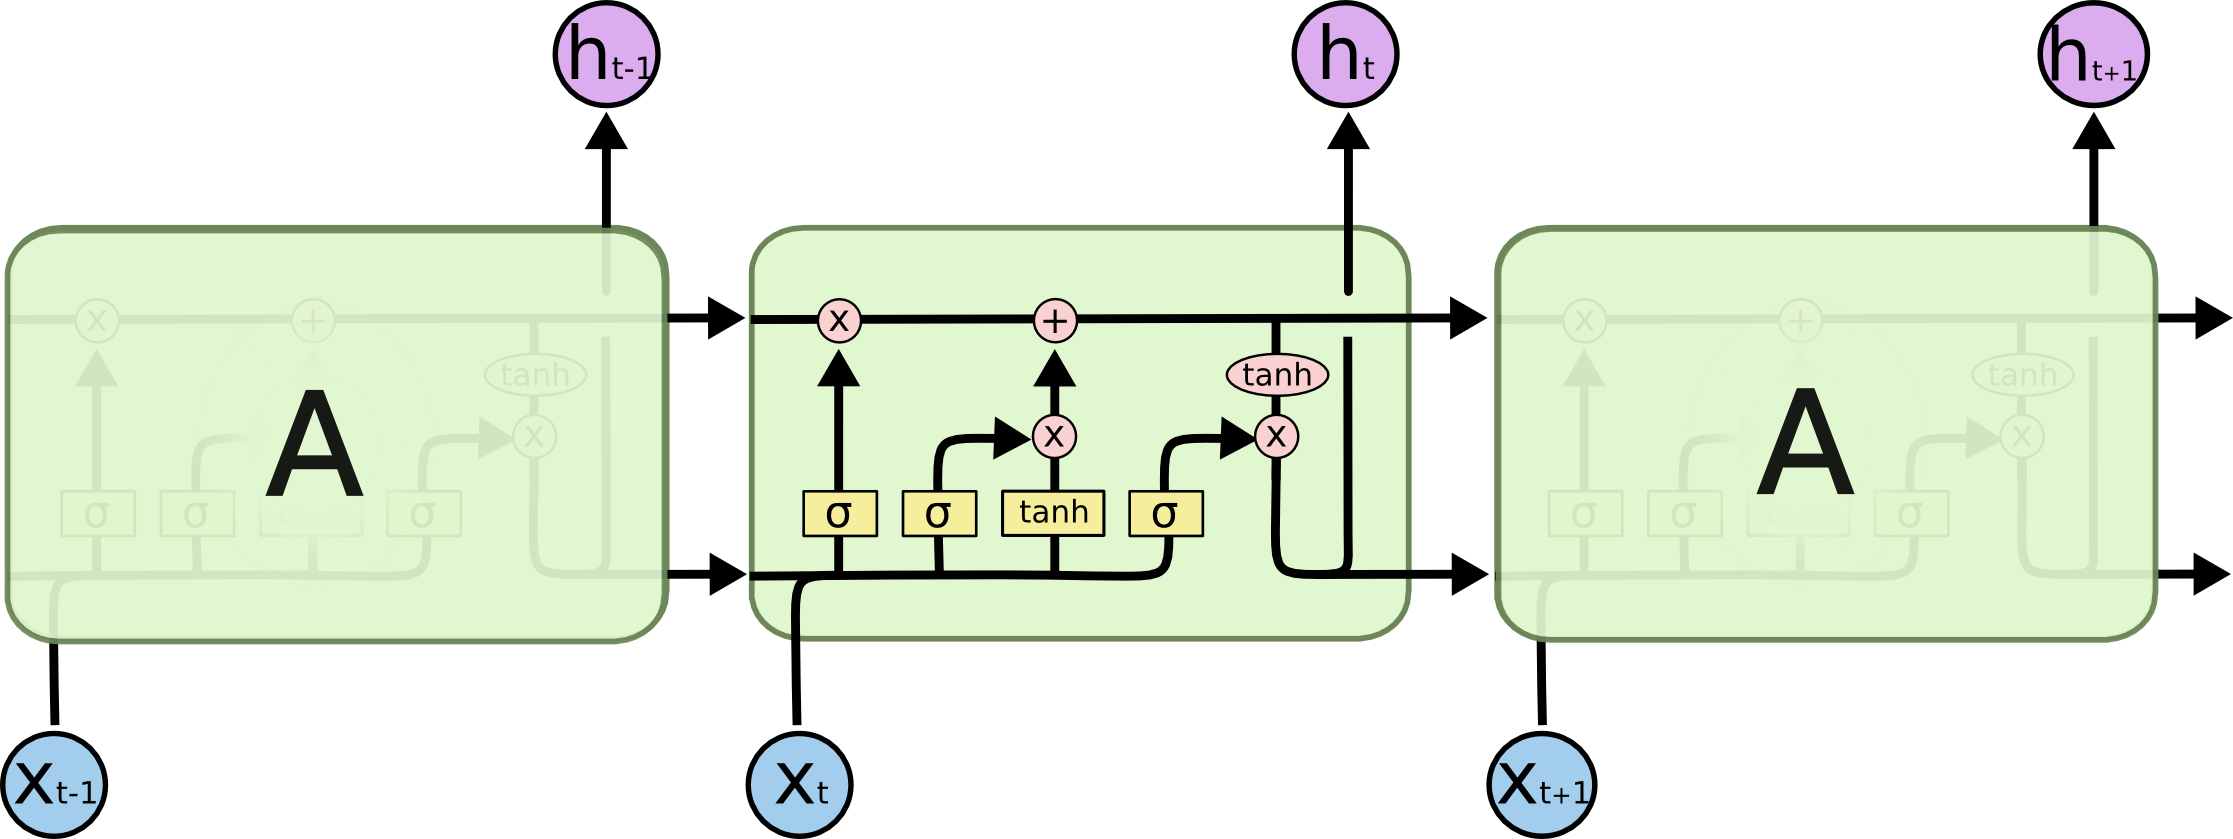
\includegraphics[width=14cm]{./Chapitre3/figures/lstm.png}
  \caption{Représentation schématique d'un réseau récurrent à mémoire court et long terme (LSTM). On observe qu'il y a deux entrées à l'unité neuronale : l'état de la cellule (cell state) en haut et la sortie classique d'un neurone en bas. Image provenant de http://colah.github.io/posts/2015-08-Understanding-LSTMs/ .}
  \label{fig:lstm}
\end{figure}
